\chapter{User Manual}
\label{user manual}

%Installation
\section*{Installation}

\subsection*{System Requirements}
The system has been designed and tested on a portable computing system, and thus should operate effectively on a modern laptop. The minimum recommended requirements are as follows: \\

\begin{itemize}
    \item Operating System: Microsoft Windows 7
    \item Processor: 1.5GHz Dual-core x86/x64
    \item Memory: 4GB
    \item Hard Drive: 20GB free
    \item USB Drive/Internet Connectivity/CD Drive (for installation)
    \item Xbox Kinect / Microsoft Kinect device
\end{itemize} \\

\subsection*{Kinect}
The majority of the functionality requires that an Xbox Kinect is installed and present on the system. This requires the installation of the Kinect for Windows drivers, which should occur automatically once the device has been plugged in for the first time. 

\subsection*{Software}
The software can be installed by dragging and dropping the contents from the installation media into a suitable directory on the computer where the software is intended to be deployed. %or packaging it up in the form of an installer, vs2010 supports this? bernie

%Usage
\section*{Entering a New Patient}
From the "Welcome" menu, select "Add New Patient".\\

\begin{figure}[h]
\begin{center}
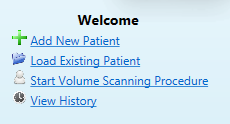
\includegraphics[scale=1]{images/welcome}
\end{center}
\caption{The Welcome menu}
\label{the welcome menu}
\end{figure}

Input the patients details and click "Proceed". The add any relevant conditions and click "Proceed and Save".\\

\begin{figure}[h]
\begin{center}
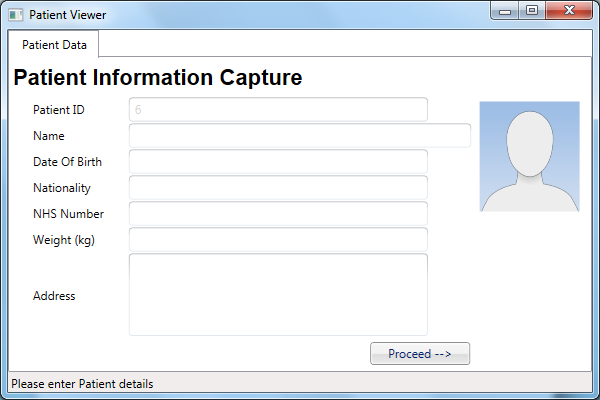
\includegraphics[scale=0.6]{images/details}
\end{center}
\caption{First stage of patient entry}
\label{first stage of patient entry}
\end{figure}

\begin{figure}[!h]
\begin{center}
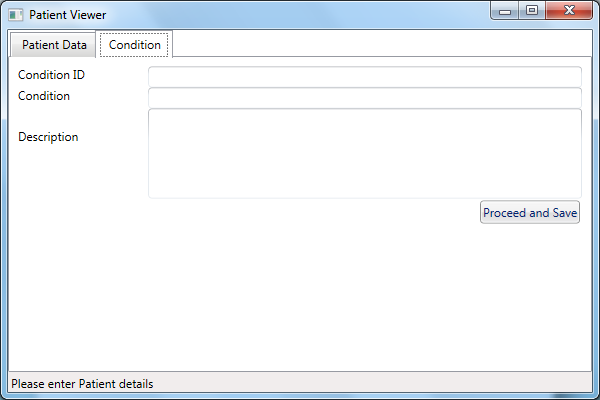
\includegraphics[scale=0.6]{images/details2}
\end{center}
\caption{Second stage of patient entry}
\label{second stage of patient entry}
\end{figure}


\begin{figure}[h]
\begin{center}
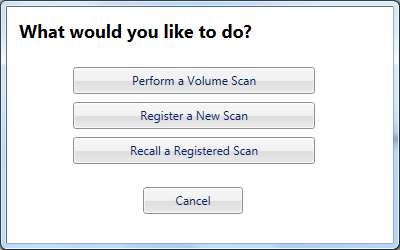
\includegraphics[scale=0.6]{images/scans}
\end{center}
\caption{The scan options available in the PARSE toolkit.}
\label{scans}
\end{figure}

\section*{Loading an Old Patient}
From the "Welcome" menu, select "Load Existing Patient".\\

\begin{figure}[h]
\begin{center}
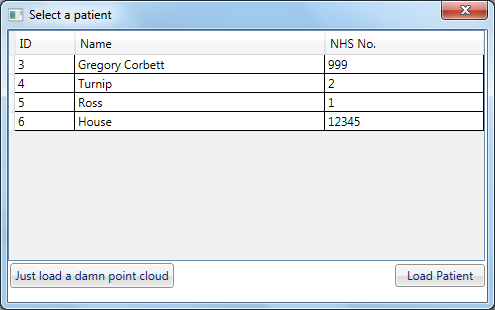
\includegraphics[scale=0.6]{images/old}
\end{center}
\caption{Load existing patient}
\label{load existing patient}
\end{figure}

\section*{Adding a measurement with a handheld sensor}
Ensure that you have your PARSE certified sensing device ready. Then, from the main menu select Patient $>$ Add Markerless Scan. A new window will appear as below. When ready, click to start the scan process.\\
\begin{Description}
\item[Stand in view] Both you and the patient should stand in view of the Kinect device, such that you fit well within the on-screen picture.
\item[Show the sensor] The program will search for the sensing device, and use it to identify the doctor - hold it in one hand and present it clearly to the device, away from the patient.
\item[Move a little] Sometimes the program may have difficulty distinguishing people from the environment. In this case, move around a little to hasten the process.
\item[Take your measurement] Holding the transducer still for several seconds will automatically trigger the capture process. Take your measurement, and then hold the scanner still until the window closes. When the window closes, the measurement has been taken and the position recorded. 

\section{Recording a Scan}

Upon entering patient details, you will be able to select from a possible number of scan types. Select the `Perform a Volume Scan' option. You will then be presented with the Scan Loader interface. At this point, calibrate the patient in front of the scanner. A skeleton overlay will display and the colour of the skeleton will correspond to the suitable depth that the skeleton needs to be at for scanning. If the subject is {\color{blue}too close}, the skeleton will be instructed to move away. If the subject is {\color{red}too far}, the skeleton will be instructed to move closer. The optimal position will be highlighted when the skeleton becomes {\color{green}green}. \\

At this point, the patient will be instructed to rotate on the spot 4 times in order to capture the scan. The scan will then be rendered and visualised. \\

\begin{figure}[h]
\begin{center}
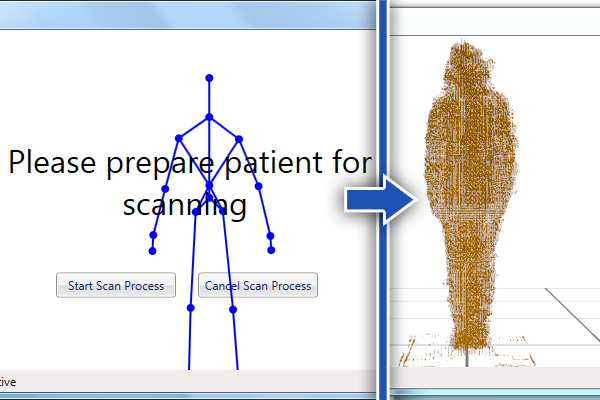
\includegraphics[scale=0.6]{zscreenshots/ScanViewer_Combi.png}
\end{center}
\caption{Patient Scanning Dialog followed by Scan Visualisation}
\label{combination of scanviewers}
\end{figure}

\section{Calculating Body Measurements}

The PARSE toolkit is capable of calculating volume and limb circumference as well as other detailed metrics such as BMI and body fat percentage. To calculate the volume of a scan, click the `Calculate Volume' option in the `Patient Options' menu item. A dialog will then load and show the volume of the patient along with a visualisation for each plane and other metrics such as BMI and Body fat percentage based on their calculated volume. \\

Limb Circumference is calculated by selecting the `Limb Circumference' option. The Limb Circumference detail view will then load and each limb can be selected using a drop down box. The limb circumference is also visualised for each limb selected. Historic limb circumference scans visualisations can then be selected and viewed alongside the most recent scan visualisation. \\

\begin{figure}[!h]
\begin{center}
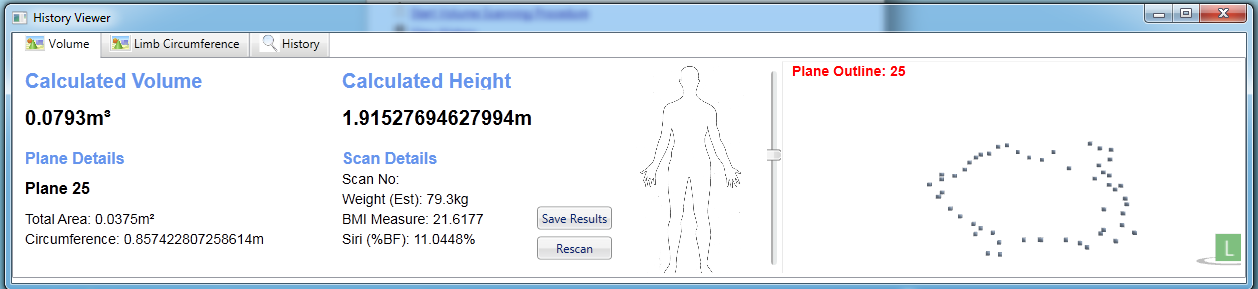
\includegraphics[scale=0.35]{zscreenshots/voldetail.png}
\end{center}
\caption{The volume detail dialog after calculation}
\label{volume detail}
\end{figure}

\begin{figure}[!h]
\begin{center}
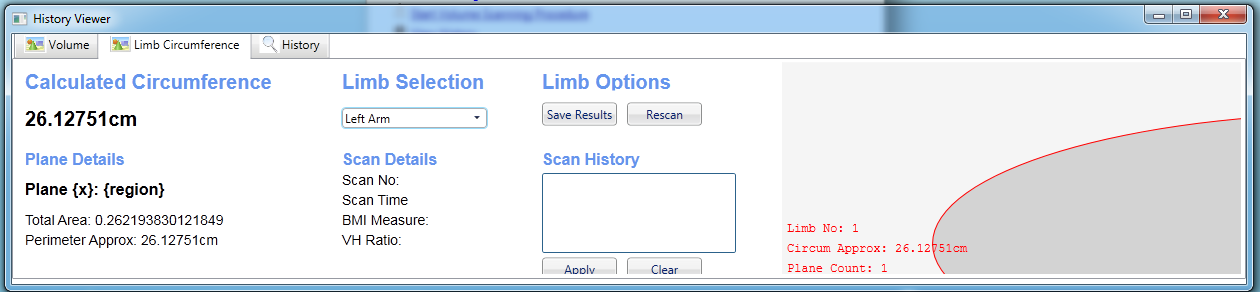
\includegraphics[scale=0.35]{zscreenshots/circumdetail.png}
\end{center}
\caption{The limb circumference dialog after calculation}
\label{limb circumference detail}
\end{figure}


\section{Additional Options}

\subsection{Scan Refinement}

In the instance that the Kinect captures too much of the ground plane from the scan. There are additional options to refine the point cloud so as to generate a more accurate series of calculations. Select Scan Refinement and then proceed to select 'Remove Ground Plane'. This will then re-render the model with the ground plane removed in the instance that excessive amounts of floor have been captured.

\subsection{Saving .PARSE or .PCD Files}

Scans can be saved in the proprietary .PARSE format or in a more standard .PCD format so that scans can then be incorporated into the Point Cloud Library for further point cloud processing. This allows for further refinements or better registration of the point cloud to take place. Select the `Export' option and then select Export to .PARSE or Export to .PCD.

\subsection{Loading .PARSE or .PCD Files}

There is an option to reload .PARSE files but also .PCD files. This means that point cloud reconstructions that have been produced using the point cloud library can be subject to volume and limb circumference calculations if required and this provides an intermeidary solution if our scanning mechanism produces an innacurate scan. These point could files can be loaded selecting the 'Load Scans' option.

\subsection{Deleting or Editing Patient Records}

The editing and deletion of patient records takes place in the Patient Viewer. For each patient, there is an option to either edit or delete the record by selecting the 'Edit' or 'Delete' option on the Patient Information Viewer. If the patient is deleted, all the associated results and scans will also be deleted.

